\documentclass[]{article}
\usepackage{lmodern}
\usepackage{amssymb,amsmath}
\usepackage{ifxetex,ifluatex}
\usepackage{fixltx2e} % provides \textsubscript
\ifnum 0\ifxetex 1\fi\ifluatex 1\fi=0 % if pdftex
  \usepackage[T1]{fontenc}
  \usepackage[utf8]{inputenc}
\else % if luatex or xelatex
  \ifxetex
    \usepackage{mathspec}
  \else
    \usepackage{fontspec}
  \fi
  \defaultfontfeatures{Ligatures=TeX,Scale=MatchLowercase}
\fi
% use upquote if available, for straight quotes in verbatim environments
\IfFileExists{upquote.sty}{\usepackage{upquote}}{}
% use microtype if available
\IfFileExists{microtype.sty}{%
\usepackage{microtype}
\UseMicrotypeSet[protrusion]{basicmath} % disable protrusion for tt fonts
}{}
\usepackage[margin=1in]{geometry}
\usepackage{hyperref}
\hypersetup{unicode=true,
            pdftitle={Classification algorithm - Neural Networks},
            pdfauthor={Eric Roseren},
            pdfborder={0 0 0},
            breaklinks=true}
\urlstyle{same}  % don't use monospace font for urls
\usepackage{color}
\usepackage{fancyvrb}
\newcommand{\VerbBar}{|}
\newcommand{\VERB}{\Verb[commandchars=\\\{\}]}
\DefineVerbatimEnvironment{Highlighting}{Verbatim}{commandchars=\\\{\}}
% Add ',fontsize=\small' for more characters per line
\usepackage{framed}
\definecolor{shadecolor}{RGB}{248,248,248}
\newenvironment{Shaded}{\begin{snugshade}}{\end{snugshade}}
\newcommand{\KeywordTok}[1]{\textcolor[rgb]{0.13,0.29,0.53}{\textbf{#1}}}
\newcommand{\DataTypeTok}[1]{\textcolor[rgb]{0.13,0.29,0.53}{#1}}
\newcommand{\DecValTok}[1]{\textcolor[rgb]{0.00,0.00,0.81}{#1}}
\newcommand{\BaseNTok}[1]{\textcolor[rgb]{0.00,0.00,0.81}{#1}}
\newcommand{\FloatTok}[1]{\textcolor[rgb]{0.00,0.00,0.81}{#1}}
\newcommand{\ConstantTok}[1]{\textcolor[rgb]{0.00,0.00,0.00}{#1}}
\newcommand{\CharTok}[1]{\textcolor[rgb]{0.31,0.60,0.02}{#1}}
\newcommand{\SpecialCharTok}[1]{\textcolor[rgb]{0.00,0.00,0.00}{#1}}
\newcommand{\StringTok}[1]{\textcolor[rgb]{0.31,0.60,0.02}{#1}}
\newcommand{\VerbatimStringTok}[1]{\textcolor[rgb]{0.31,0.60,0.02}{#1}}
\newcommand{\SpecialStringTok}[1]{\textcolor[rgb]{0.31,0.60,0.02}{#1}}
\newcommand{\ImportTok}[1]{#1}
\newcommand{\CommentTok}[1]{\textcolor[rgb]{0.56,0.35,0.01}{\textit{#1}}}
\newcommand{\DocumentationTok}[1]{\textcolor[rgb]{0.56,0.35,0.01}{\textbf{\textit{#1}}}}
\newcommand{\AnnotationTok}[1]{\textcolor[rgb]{0.56,0.35,0.01}{\textbf{\textit{#1}}}}
\newcommand{\CommentVarTok}[1]{\textcolor[rgb]{0.56,0.35,0.01}{\textbf{\textit{#1}}}}
\newcommand{\OtherTok}[1]{\textcolor[rgb]{0.56,0.35,0.01}{#1}}
\newcommand{\FunctionTok}[1]{\textcolor[rgb]{0.00,0.00,0.00}{#1}}
\newcommand{\VariableTok}[1]{\textcolor[rgb]{0.00,0.00,0.00}{#1}}
\newcommand{\ControlFlowTok}[1]{\textcolor[rgb]{0.13,0.29,0.53}{\textbf{#1}}}
\newcommand{\OperatorTok}[1]{\textcolor[rgb]{0.81,0.36,0.00}{\textbf{#1}}}
\newcommand{\BuiltInTok}[1]{#1}
\newcommand{\ExtensionTok}[1]{#1}
\newcommand{\PreprocessorTok}[1]{\textcolor[rgb]{0.56,0.35,0.01}{\textit{#1}}}
\newcommand{\AttributeTok}[1]{\textcolor[rgb]{0.77,0.63,0.00}{#1}}
\newcommand{\RegionMarkerTok}[1]{#1}
\newcommand{\InformationTok}[1]{\textcolor[rgb]{0.56,0.35,0.01}{\textbf{\textit{#1}}}}
\newcommand{\WarningTok}[1]{\textcolor[rgb]{0.56,0.35,0.01}{\textbf{\textit{#1}}}}
\newcommand{\AlertTok}[1]{\textcolor[rgb]{0.94,0.16,0.16}{#1}}
\newcommand{\ErrorTok}[1]{\textcolor[rgb]{0.64,0.00,0.00}{\textbf{#1}}}
\newcommand{\NormalTok}[1]{#1}
\usepackage{graphicx,grffile}
\makeatletter
\def\maxwidth{\ifdim\Gin@nat@width>\linewidth\linewidth\else\Gin@nat@width\fi}
\def\maxheight{\ifdim\Gin@nat@height>\textheight\textheight\else\Gin@nat@height\fi}
\makeatother
% Scale images if necessary, so that they will not overflow the page
% margins by default, and it is still possible to overwrite the defaults
% using explicit options in \includegraphics[width, height, ...]{}
\setkeys{Gin}{width=\maxwidth,height=\maxheight,keepaspectratio}
\IfFileExists{parskip.sty}{%
\usepackage{parskip}
}{% else
\setlength{\parindent}{0pt}
\setlength{\parskip}{6pt plus 2pt minus 1pt}
}
\setlength{\emergencystretch}{3em}  % prevent overfull lines
\providecommand{\tightlist}{%
  \setlength{\itemsep}{0pt}\setlength{\parskip}{0pt}}
\setcounter{secnumdepth}{0}
% Redefines (sub)paragraphs to behave more like sections
\ifx\paragraph\undefined\else
\let\oldparagraph\paragraph
\renewcommand{\paragraph}[1]{\oldparagraph{#1}\mbox{}}
\fi
\ifx\subparagraph\undefined\else
\let\oldsubparagraph\subparagraph
\renewcommand{\subparagraph}[1]{\oldsubparagraph{#1}\mbox{}}
\fi

%%% Use protect on footnotes to avoid problems with footnotes in titles
\let\rmarkdownfootnote\footnote%
\def\footnote{\protect\rmarkdownfootnote}

%%% Change title format to be more compact
\usepackage{titling}

% Create subtitle command for use in maketitle
\providecommand{\subtitle}[1]{
  \posttitle{
    \begin{center}\large#1\end{center}
    }
}

\setlength{\droptitle}{-2em}

  \title{Classification algorithm - Neural Networks}
    \pretitle{\vspace{\droptitle}\centering\huge}
  \posttitle{\par}
    \author{Eric Roseren}
    \preauthor{\centering\large\emph}
  \postauthor{\par}
      \predate{\centering\large\emph}
  \postdate{\par}
    \date{5/9/2019}


\begin{document}
\maketitle

\subsection{Introduction}\label{introduction}

In this section we will implement an L-layer neural network from scratch
and use it for classification tasks.

To load a dataset that is stored on an H5 file we can use the rhdf5
package from Bioconductor as follow:

\begin{Shaded}
\begin{Highlighting}[]
\CommentTok{#source("http://bioconductor.org/biocLite.R") # Install package from bioconductor source}
\CommentTok{#biocLite("rhdf5")}
\KeywordTok{library}\NormalTok{(rhdf5) }\CommentTok{# load package }
\KeywordTok{library}\NormalTok{(countcolors)  }\CommentTok{# plot (rgb array)}
\end{Highlighting}
\end{Shaded}

\begin{verbatim}
## Warning: package 'countcolors' was built under R version 3.5.2
\end{verbatim}

Guidelines: *List the objects within the file to find the data group you
want to read:

\begin{Shaded}
\begin{Highlighting}[]
\CommentTok{#h5ls("train_catvnoncat.h5")}
\NormalTok{f <-}\StringTok{ "train_catvnoncat.h5"}
\CommentTok{# view the structure of the H5 file}
\KeywordTok{h5ls}\NormalTok{(f, }\DataTypeTok{all =} \OtherTok{TRUE}\NormalTok{)}
\end{Highlighting}
\end{Shaded}

\begin{verbatim}
##   group         name         ltype corder_valid corder cset       otype
## 0     / list_classes H5L_TYPE_HARD        FALSE      0    0 H5I_DATASET
## 1     /  train_set_x H5L_TYPE_HARD        FALSE      0    0 H5I_DATASET
## 2     /  train_set_y H5L_TYPE_HARD        FALSE      0    0 H5I_DATASET
##   num_attrs  dclass         dtype  stype rank               dim
## 0         0  STRING    HST_STRING SIMPLE    1                 2
## 1         0 INTEGER  H5T_STD_U8LE SIMPLE    4 3 x 64 x 64 x 209
## 2         0 INTEGER H5T_STD_I64LE SIMPLE    1               209
##              maxdim
## 0                 2
## 1 3 x 64 x 64 x 209
## 2               209
\end{verbatim}

*Read the HDF5 data:

\begin{Shaded}
\begin{Highlighting}[]
\NormalTok{load.dataset <-}\StringTok{ }\ControlFlowTok{function}\NormalTok{()\{}
\CommentTok{#Standardised training set}
\NormalTok{train.x <-}\StringTok{ }\KeywordTok{aperm}\NormalTok{(}\KeywordTok{h5read}\NormalTok{(}\StringTok{"train_catvnoncat.h5"}\NormalTok{,}\StringTok{"train_set_x"}\NormalTok{))}\OperatorTok{/}\DecValTok{255}
\NormalTok{train.y <-}\StringTok{ }\KeywordTok{t}\NormalTok{(}\KeywordTok{h5read}\NormalTok{(}\StringTok{"train_catvnoncat.h5"}\NormalTok{,}\StringTok{"train_set_y"}\NormalTok{))}


\CommentTok{# Standardised test set}
\NormalTok{test.x <-}\StringTok{ }\KeywordTok{aperm}\NormalTok{(}\KeywordTok{h5read}\NormalTok{(}\StringTok{"test_catvnoncat.h5"}\NormalTok{,}\StringTok{"test_set_x"}\NormalTok{))}\OperatorTok{/}\DecValTok{255}
\NormalTok{test.y <-}\StringTok{ }\KeywordTok{t}\NormalTok{(}\KeywordTok{h5read}\NormalTok{(}\StringTok{"test_catvnoncat.h5"}\NormalTok{,}\StringTok{"test_set_y"}\NormalTok{))}

\CommentTok{# classes }

\NormalTok{classes =}\StringTok{ }\KeywordTok{h5read}\NormalTok{(}\StringTok{"test_catvnoncat.h5"}\NormalTok{,}\StringTok{"list_classes"}\NormalTok{)}
\NormalTok{output <-}\StringTok{ }\KeywordTok{list}\NormalTok{(}\DataTypeTok{train.x=}\NormalTok{train.x,}\DataTypeTok{train.y=}\NormalTok{train.y,}
               \DataTypeTok{test.x=}\NormalTok{test.x,}\DataTypeTok{test.y=}\NormalTok{test.y,}\DataTypeTok{classes=}\NormalTok{classes)}
\KeywordTok{return}\NormalTok{(output)}
\NormalTok{\}}
\end{Highlighting}
\end{Shaded}

\begin{Shaded}
\begin{Highlighting}[]
\NormalTok{original.data <-}\StringTok{ }\KeywordTok{load.dataset}\NormalTok{()}
\end{Highlighting}
\end{Shaded}

\subsection{The data}\label{the-data}

To represent color images, the red, green and blue channels (RGB) must
be specified for each pixel, and so the pixel value is actually a vector
of three numbers ranging from 0 to 255.

One common preprocessing step in machine learning is to center and
standardize your dataset, meaning that you substract the mean of the
whole numpy array from each example, and then divide each example by the
standard deviation of the whole numpy array. But for picture datasets,
it is simpler and more convenient and works almost as well to just
divide every row of the dataset by 255 (the maximum value of a pixel
channel).

Let's visualise the 25th image:

\begin{Shaded}
\begin{Highlighting}[]
\NormalTok{index <-}\StringTok{ }\DecValTok{23}
\NormalTok{m <-}\StringTok{ }\NormalTok{original.data}\OperatorTok{$}\NormalTok{train.x[index,,,]}
\NormalTok{result <-}\KeywordTok{as.numeric}\NormalTok{( }\KeywordTok{t}\NormalTok{(original.data}\OperatorTok{$}\NormalTok{train.y[index]))}
\NormalTok{cat.noncat <-}\StringTok{ }\NormalTok{original.data}\OperatorTok{$}\NormalTok{classes[result}\OperatorTok{+}\DecValTok{1}\NormalTok{]}
\KeywordTok{plotArrayAsImage}\NormalTok{(m, }\DataTypeTok{main =} \KeywordTok{paste}\NormalTok{(}\StringTok{"y= "}\NormalTok{,result,}\StringTok{", it is a "}\NormalTok{,cat.noncat,}\StringTok{" image "}\NormalTok{,}\DataTypeTok{sep =} \StringTok{""}\NormalTok{ ))}
\end{Highlighting}
\end{Shaded}

\includegraphics{Neural_Networks_in_R_files/figure-latex/unnamed-chunk-5-1.pdf}

We will be performing a multitude of matrix multiplication so having in
mind the dimensions of the data training and test set will be helpful.

\begin{Shaded}
\begin{Highlighting}[]
\NormalTok{m.train <-}\StringTok{ }\KeywordTok{dim}\NormalTok{(original.data}\OperatorTok{$}\NormalTok{train.x)[}\DecValTok{1}\NormalTok{]}
\NormalTok{m.test <-}\StringTok{ }\KeywordTok{dim}\NormalTok{(original.data}\OperatorTok{$}\NormalTok{test.x)[}\DecValTok{1}\NormalTok{]}
\NormalTok{num.px <-}\StringTok{ }\KeywordTok{dim}\NormalTok{(original.data}\OperatorTok{$}\NormalTok{train.x)[}\DecValTok{2}\NormalTok{]}
\end{Highlighting}
\end{Shaded}

Remember that train.set.x is an array of shape (m.train, num.px, num.px,
3). To feed the images to the neural network, the dimension of the array
needs to be flatten. The dimension of the new array will have the
following shape: (num.px \(*\) num.px \(*\) 3, 1).

\begin{Shaded}
\begin{Highlighting}[]
\NormalTok{train.x.flatten <-}\StringTok{ }\KeywordTok{matrix}\NormalTok{(}\DataTypeTok{data =} \KeywordTok{aperm}\NormalTok{(original.data}\OperatorTok{$}\NormalTok{train.x),num.px}\OperatorTok{*}\NormalTok{num.px}\OperatorTok{*}\DecValTok{3}\NormalTok{,m.train)}
\NormalTok{test.x.flatten <-}\StringTok{ }\KeywordTok{matrix}\NormalTok{(}\DataTypeTok{data =} \KeywordTok{aperm}\NormalTok{(original.data}\OperatorTok{$}\NormalTok{test.x),num.px}\OperatorTok{*}\NormalTok{num.px}\OperatorTok{*}\DecValTok{3}\NormalTok{,m.test)}
\end{Highlighting}
\end{Shaded}

\subsection{General Architecture of the learning
algorithm}\label{general-architecture-of-the-learning-algorithm}

The following Figure explains why Logistic Regression is actually a very
simple Neural Network!
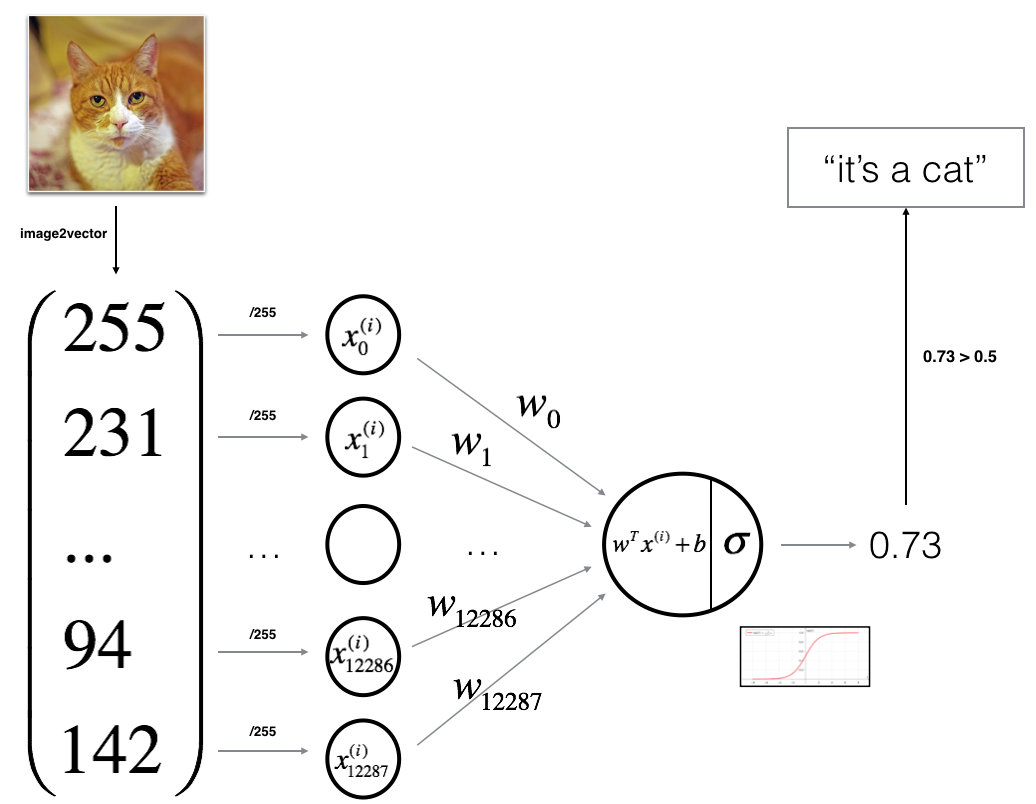
\includegraphics{/users/eric/Documents/R programming/Classification-algorithms/figure/LogReg_kiank.png}
\textbf{Mathematical expression of the algorithm}:

For one example \(x^{(i)}\): \[z^{(i)} = w^T x^{(i)} + b \tag{1}\]
\[\hat{y}^{(i)} = a^{(i)} = sigmoid(z^{(i)})\tag{2}\]
\[ \mathcal{L}(a^{(i)}, y^{(i)}) =  - y^{(i)}  \log(a^{(i)}) - (1-y^{(i)} )  \log(1-a^{(i)})\tag{3}\]

The cost is then computed by summing over all training examples:
\[ J = \frac{1}{m} \sum_{i=1}^m \mathcal{L}(a^{(i)}, y^{(i)})\tag{6}\]

\subsection{4 - Building the parts of our
algorithm}\label{building-the-parts-of-our-algorithm}

The main steps for building a Neural Network are: \emph{1. Define the
model structure (such as number of input features) }2. Initialize the
model's parameters *3. Loop: - Calculate current loss (forward
propagation) - Calculate current gradient (backward propagation) -
Update parameters (gradient descent)

\begin{Shaded}
\begin{Highlighting}[]
\CommentTok{# Sigmoid function}

\NormalTok{sigmoid <-}\StringTok{ }\ControlFlowTok{function}\NormalTok{(z)\{}
  \StringTok{"}
\StringTok{    Compute the sigmoid of z}

\StringTok{    Arguments:}
\StringTok{    z -- A scalar or array of any size.}

\StringTok{    Return:}
\StringTok{    s -- sigmoid(z)}
\StringTok{    "}
\NormalTok{  s <-}\StringTok{ }\DecValTok{1}\OperatorTok{/}\NormalTok{(}\DecValTok{1}\OperatorTok{+}\KeywordTok{exp}\NormalTok{(}\OperatorTok{-}\NormalTok{z))}
  \KeywordTok{return}\NormalTok{(s)}
\NormalTok{\}}
\end{Highlighting}
\end{Shaded}

\begin{Shaded}
\begin{Highlighting}[]
\KeywordTok{print}\NormalTok{ (}\KeywordTok{paste}\NormalTok{(}\StringTok{"sigmoid([0, 2]) = "}\NormalTok{, }\KeywordTok{as.numeric}\NormalTok{(}\KeywordTok{sigmoid}\NormalTok{(}\KeywordTok{array}\NormalTok{(}\DataTypeTok{data=}\KeywordTok{c}\NormalTok{(}\DecValTok{0}\NormalTok{,}\DecValTok{2}\NormalTok{)))),}\DataTypeTok{sep =} \StringTok{""}\NormalTok{))}
\end{Highlighting}
\end{Shaded}

\begin{verbatim}
## [1] "sigmoid([0, 2]) = 0.5"              
## [2] "sigmoid([0, 2]) = 0.880797077977882"
\end{verbatim}

\subsubsection{4.2 - Initializing
parameters}\label{initializing-parameters}

We need to initialise the parameters w and b to zero:

\begin{Shaded}
\begin{Highlighting}[]
\NormalTok{initialise.to.zero <-}\StringTok{ }\ControlFlowTok{function}\NormalTok{(shape)\{}
  \StringTok{"}
\StringTok{    This function creates a vector of zeros of dimension (shape, 1) for w and initializes b to 0.}
\StringTok{    }
\StringTok{    Argument:}
\StringTok{    dim -- size of the w vector we want (or number of parameters in this case)}
\StringTok{    }
\StringTok{    Returns:}
\StringTok{    w -- initialized vector of shape (dim, 1)}
\StringTok{    b -- initialized scalar (corresponds to the bias)}
\StringTok{    "}
\NormalTok{ w <-}\StringTok{ }\KeywordTok{matrix}\NormalTok{(}\DataTypeTok{data =} \KeywordTok{rep}\NormalTok{(}\DecValTok{0}\NormalTok{,shape),}\DataTypeTok{nrow =}\NormalTok{ shape,}\DataTypeTok{ncol =} \DecValTok{1}\NormalTok{) }
\NormalTok{ b <-}\StringTok{ }\DecValTok{0}
\NormalTok{ result <-}\StringTok{ }\KeywordTok{list}\NormalTok{(}\DataTypeTok{w=}\NormalTok{w,}\DataTypeTok{b=}\NormalTok{b)}
 \KeywordTok{return}\NormalTok{(result)}
\NormalTok{\}}
\end{Highlighting}
\end{Shaded}

\subsubsection{4.3 - Forward and Backward
propagation}\label{forward-and-backward-propagation}

Forward Propagation: * get X *
\[A = \sigma(w^T X + b) = (a^{(1)}, a^{(2)}, ..., a^{(m-1)}, a^{(m)})\]
* You calculate the cost function:
\[J = \frac{1}{m}\sum_{i=1}^{m}y^{(i)}\log(a^{(i)})+(1-y^{(i)})\log(1-a^{(i)})\]

Here are the two formulas :

\[ \frac{\partial J}{\partial w} = \frac{1}{m}X(A-Y)^T\tag{7}\]
\[ \frac{\partial J}{\partial b} = \frac{1}{m} \sum_{i=1}^m (a^{(i)}-y^{(i)})\tag{8}\]

\begin{Shaded}
\begin{Highlighting}[]
\NormalTok{propagate <-}\StringTok{ }\ControlFlowTok{function}\NormalTok{(w, b, X, Y)\{}
    \StringTok{"}
\StringTok{    Implement the cost function and its gradient for the propagation explained above}

\StringTok{    Arguments:}
\StringTok{    w -- weights, a numpy array of size (num_px * num_px * 3, 1)}
\StringTok{    b -- bias, a scalar}
\StringTok{    X -- data of size (num_px * num_px * 3, number of examples)}
\StringTok{    Y -- true label vector (containing 0 if non-cat, 1 if cat) of size (1, number of examples)}

\StringTok{    Return:}
\StringTok{    cost -- negative log-likelihood cost for logistic regression}
\StringTok{    dw -- gradient of the loss with respect to w, thus same shape as w}
\StringTok{    db -- gradient of the loss with respect to b, thus same shape as b}
\StringTok{    }

\StringTok{    "}
    
\NormalTok{    m <-}\StringTok{  }\KeywordTok{dim}\NormalTok{(X)[}\DecValTok{2}\NormalTok{]}
    
    \CommentTok{# FORWARD PROPAGATION (FROM X TO COST)}
\NormalTok{    A <-}\StringTok{ }\KeywordTok{sigmoid}\NormalTok{((}\KeywordTok{t}\NormalTok{(w) }\OperatorTok\StringTok{ }\NormalTok{X)}\OperatorTok{+}\NormalTok{b)                                    }\CommentTok{# compute activation}
\NormalTok{    cost <-}\StringTok{ }\NormalTok{(}\OperatorTok{-}\DecValTok{1}\OperatorTok{/}\NormalTok{m)}\OperatorTok{*}\KeywordTok{sum}\NormalTok{(Y}\OperatorTok{*}\KeywordTok{log}\NormalTok{(A)}\OperatorTok{+}\NormalTok{(}\DecValTok{1}\OperatorTok{-}\NormalTok{Y)}\OperatorTok{*}\KeywordTok{log}\NormalTok{(}\DecValTok{1}\OperatorTok{-}\NormalTok{A))                                 }\CommentTok{# compute cost}

    \CommentTok{# BACKWARD PROPAGATION (TO FIND GRAD)}
\NormalTok{    dw <-}\StringTok{  }\NormalTok{(}\DecValTok{1}\OperatorTok{/}\NormalTok{m)}\OperatorTok{*}\NormalTok{X }\OperatorTok\StringTok{ }\KeywordTok{t}\NormalTok{((A}\OperatorTok{-}\NormalTok{Y))}
\NormalTok{    db <-}\StringTok{  }\NormalTok{(}\DecValTok{1}\OperatorTok{/}\NormalTok{m)}\OperatorTok{*}\KeywordTok{sum}\NormalTok{(A}\OperatorTok{-}\NormalTok{Y)}

    \KeywordTok{stopifnot}\NormalTok{(}\KeywordTok{dim}\NormalTok{(dw) }\OperatorTok{==}\StringTok{ }\KeywordTok{dim}\NormalTok{(w))}
    
    \CommentTok{#cost <-  np.squeeze(cost)}
    
\NormalTok{    grads =}\StringTok{ }\KeywordTok{list}\NormalTok{(}\DataTypeTok{dw=}\NormalTok{dw,}\DataTypeTok{db=}\NormalTok{db)}
    
\NormalTok{    results <-}\StringTok{ }\KeywordTok{list}\NormalTok{(}\DataTypeTok{grads=}\NormalTok{grads,}\DataTypeTok{cost=}\NormalTok{cost)}
    
    \KeywordTok{return}\NormalTok{ (results)}
\NormalTok{\}}
\end{Highlighting}
\end{Shaded}

\begin{Shaded}
\begin{Highlighting}[]
\NormalTok{w <-}\StringTok{ }\KeywordTok{array}\NormalTok{(}\DataTypeTok{data =} \KeywordTok{c}\NormalTok{(}\DecValTok{1}\NormalTok{,}\DecValTok{2}\NormalTok{),}\DataTypeTok{dim =} \KeywordTok{c}\NormalTok{(}\DecValTok{2}\NormalTok{,}\DecValTok{1}\NormalTok{))}
\NormalTok{b <-}\StringTok{ }\DecValTok{2}
\NormalTok{X <-}\StringTok{ }\KeywordTok{array}\NormalTok{(}\DataTypeTok{data =}\KeywordTok{c}\NormalTok{(}\DecValTok{1}\NormalTok{,}\DecValTok{3}\NormalTok{,}\DecValTok{2}\NormalTok{,}\DecValTok{4}\NormalTok{,}\OperatorTok{-}\DecValTok{1}\NormalTok{,}\OperatorTok{-}\FloatTok{3.2}\NormalTok{),}\DataTypeTok{dim =} \KeywordTok{c}\NormalTok{(}\DecValTok{2}\NormalTok{,}\DecValTok{3}\NormalTok{))}
\NormalTok{Y <-}\StringTok{ }\KeywordTok{array}\NormalTok{(}\DataTypeTok{data =}\KeywordTok{c}\NormalTok{(}\DecValTok{1}\NormalTok{,}\DecValTok{0}\NormalTok{,}\DecValTok{1}\NormalTok{),}\DataTypeTok{dim =} \KeywordTok{c}\NormalTok{(}\DecValTok{1}\NormalTok{,}\DecValTok{3}\NormalTok{))}

\KeywordTok{propagate}\NormalTok{(w,b,X,Y)}
\end{Highlighting}
\end{Shaded}

\begin{verbatim}
## $grads
## $grads$dw
##          [,1]
## [1,] 0.998456
## [2,] 2.395072
## 
## $grads$db
## [1] 0.001455578
## 
## 
## $cost
## [1] 5.801545
\end{verbatim}

\subsubsection{4.4 - Optimization}\label{optimization}

You have initialized your parameters.You are also able to compute a cost
function and its gradient. Now, you want to update the parameters using
gradient descent.

\begin{Shaded}
\begin{Highlighting}[]
\NormalTok{optimize <-}\StringTok{ }\ControlFlowTok{function}\NormalTok{(w, b, X, Y, num.iterations, learning.rate, }\DataTypeTok{print.cost =}\NormalTok{ F)\{}
    \StringTok{"}
\StringTok{    This function optimizes w and b by running a gradient descent algorithm}
\StringTok{    }
\StringTok{    Arguments:}
\StringTok{    w -- weights, a numpy array of size (num_px * num_px * 3, 1)}
\StringTok{    b -- bias, a scalar}
\StringTok{    X -- data of shape (num_px * num_px * 3, number of examples)}
\StringTok{    Y -- true label vector (containing 0 if non-cat, 1 if cat), of shape (1, number of examples)}
\StringTok{    num_iterations -- number of iterations of the optimization loop}
\StringTok{    learning_rate -- learning rate of the gradient descent update rule}
\StringTok{    print_cost -- True to print the loss every 100 steps}
\StringTok{    }
\StringTok{    Returns:}
\StringTok{    params -- dictionary containing the weights w and bias b}
\StringTok{    grads -- dictionary containing the gradients of the weights and bias with respect to the cost function}
\StringTok{    costs -- list of all the costs computed during the optimization, this will be used to plot the learning curve.}
\StringTok{    }
\StringTok{    Tips:}
\StringTok{    You basically need to write down two steps and iterate through them:}
\StringTok{        1) Calculate the cost and the gradient for the current parameters. Use propagate().}
\StringTok{        2) Update the parameters using gradient descent rule for w and b.}
\StringTok{    "}
    
\NormalTok{    costs =}\StringTok{ }\OtherTok{NULL}
    
    \ControlFlowTok{for}\NormalTok{ (i }\ControlFlowTok{in} \DecValTok{1}\OperatorTok{:}\NormalTok{num.iterations)\{}
        
        
        \CommentTok{# Cost and gradient calculation (≈ 1-4 lines of code)}
\NormalTok{        temp.val <-}\StringTok{ }\KeywordTok{propagate}\NormalTok{(w, b, X, Y)}
\NormalTok{        grads <-}\StringTok{  }\NormalTok{temp.val}\OperatorTok{$}\NormalTok{grads}
\NormalTok{        cost <-}\StringTok{  }\NormalTok{temp.val}\OperatorTok{$}\NormalTok{cost}

        \CommentTok{# Retrieve derivatives from grads}
\NormalTok{        dw <-}\StringTok{  }\NormalTok{grads}\OperatorTok{$}\NormalTok{dw}
\NormalTok{        db <-}\StringTok{  }\NormalTok{grads}\OperatorTok{$}\NormalTok{db}
        
        \CommentTok{# update rule (≈ 2 lines of code)}
        
\NormalTok{        w <-}\StringTok{  }\NormalTok{w}\OperatorTok{-}\NormalTok{learning.rate}\OperatorTok{*}\NormalTok{dw}
\NormalTok{        b <-}\StringTok{  }\NormalTok{b}\OperatorTok{-}\NormalTok{learning.rate}\OperatorTok{*}\NormalTok{db}

        \CommentTok{# Record the costs}
        \ControlFlowTok{if}\NormalTok{ (i }\OperatorTok\StringTok{ }\DecValTok{100} \OperatorTok{==}\StringTok{ }\DecValTok{0}\NormalTok{)\{}
\NormalTok{            costs[i] <-}\StringTok{ }\NormalTok{cost}
\NormalTok{        \}}
        \CommentTok{# Print the cost every 100 training iterations}
        \ControlFlowTok{if}\NormalTok{ (print.cost }\OperatorTok{&}\StringTok{ }\NormalTok{i }\OperatorTok\StringTok{ }\DecValTok{100} \OperatorTok{==}\StringTok{ }\DecValTok{0}\NormalTok{)\{}
            \KeywordTok{print}\NormalTok{ (}\KeywordTok{paste}\NormalTok{(}\StringTok{"Cost after iteration "}\NormalTok{, i,}\StringTok{": "}\NormalTok{,cost,}\DataTypeTok{sep =} \StringTok{""}\NormalTok{))}
\NormalTok{        \}}
\NormalTok{    \}}
    
\NormalTok{    params <-}\StringTok{  }\KeywordTok{list}\NormalTok{(}\DataTypeTok{w=}\NormalTok{ w,}\DataTypeTok{b=}\NormalTok{b)}
\NormalTok{    grads <-}\StringTok{  }\KeywordTok{list}\NormalTok{(}\DataTypeTok{dw=}\NormalTok{ dw,}\DataTypeTok{db=}\NormalTok{ db)}
    
\NormalTok{    out <-}\StringTok{ }\KeywordTok{list}\NormalTok{(}\DataTypeTok{params=}\NormalTok{params,}\DataTypeTok{grads=}\NormalTok{grads,}\DataTypeTok{cost=}\NormalTok{cost)}
    
    \KeywordTok{return}\NormalTok{ (out)}
\NormalTok{\}}
\end{Highlighting}
\end{Shaded}

\begin{Shaded}
\begin{Highlighting}[]
\KeywordTok{optimize}\NormalTok{(w, b, X, Y, }\DataTypeTok{num.iterations=} \DecValTok{100}\NormalTok{, }\DataTypeTok{learning.rate =} \FloatTok{0.009}\NormalTok{, }\DataTypeTok{print.cost =}\NormalTok{ F)}
\end{Highlighting}
\end{Shaded}

\begin{verbatim}
## $params
## $params$w
##           [,1]
## [1,] 0.1903359
## [2,] 0.1225916
## 
## $params$b
## [1] 1.92536
## 
## 
## $grads
## $grads$dw
##           [,1]
## [1,] 0.6775204
## [2,] 1.4162550
## 
## $grads$db
## [1] 0.2191945
## 
## 
## $cost
## [1] 1.078431
\end{verbatim}

The previous function will output the learned w and b. We are able to
use w and b to predict the labels for a dataset X. To implement the
\texttt{predict()} function. There are two steps to computing
predictions:

\begin{enumerate}
\def\labelenumi{\arabic{enumi}.}
\item
  Calculate \[\hat{Y} = A = \sigma(w^T X + b)\]
\item
  We convert the entries of a into 0 (if activation \textless{}= 0.5) or
  1 (if activation \textgreater{} 0.5), stores the predictions in a
  vector \texttt{Y\_prediction}.We can use an \texttt{if}/\texttt{else}
  statement in a \texttt{for} loop (though there is also a way to
  vectorize this).
\end{enumerate}

\begin{Shaded}
\begin{Highlighting}[]
\NormalTok{predict <-}\StringTok{ }\ControlFlowTok{function}\NormalTok{(w, b, X)\{}
    \StringTok{"}
\StringTok{    Predict whether the label is 0 or 1 using learned logistic regression parameters (w, b)}
\StringTok{    }
\StringTok{    Arguments:}
\StringTok{    w -- weights, a numpy array of size (num_px * num_px * 3, 1)}
\StringTok{    b -- bias, a scalar}
\StringTok{    X -- data of size (num_px * num_px * 3, number of examples)}
\StringTok{    }
\StringTok{    Returns:}
\StringTok{    Y_prediction -- a numpy array (vector) containing all predictions (0/1) for the examples in X}
\StringTok{    "}
    
\NormalTok{    m <-}\StringTok{  }\KeywordTok{dim}\NormalTok{(X)[}\DecValTok{2}\NormalTok{]}
\NormalTok{    Y.prediction <-}\StringTok{  }\KeywordTok{matrix}\NormalTok{(}\DataTypeTok{data=}\KeywordTok{rep}\NormalTok{(}\DecValTok{0}\NormalTok{,m),}\DataTypeTok{ncol =}\NormalTok{ m)}
    

    \CommentTok{# Compute vector "A" predicting the probabilities of a cat being present in the picture}

\NormalTok{    A <-}\StringTok{ }\KeywordTok{sigmoid}\NormalTok{((}\KeywordTok{t}\NormalTok{(w) }\OperatorTok\StringTok{ }\NormalTok{X)}\OperatorTok{+}\NormalTok{b)                                    }\CommentTok{# compute activation}

    \ControlFlowTok{for}\NormalTok{ (i }\ControlFlowTok{in} \DecValTok{1}\OperatorTok{:}\NormalTok{m)\{}
        
        \CommentTok{# Convert probabilities A[1,i] to actual predictions p[1,i]}
        \ControlFlowTok{if}\NormalTok{ (A[}\DecValTok{1}\NormalTok{,i]}\OperatorTok{>}\StringTok{ }\FloatTok{0.5}\NormalTok{)\{}
\NormalTok{            Y.prediction[}\DecValTok{1}\NormalTok{,i] <-}\StringTok{ }\DecValTok{1}
\NormalTok{        \}}
        \ControlFlowTok{else}\NormalTok{\{}
\NormalTok{            Y.prediction[}\DecValTok{1}\NormalTok{,i] <-}\StringTok{ }\DecValTok{0}
\NormalTok{        \}}
\NormalTok{    \}}

    \KeywordTok{return}\NormalTok{ (Y.prediction)}
\NormalTok{\}}
\end{Highlighting}
\end{Shaded}

\begin{Shaded}
\begin{Highlighting}[]
\NormalTok{w <-}\StringTok{ }\KeywordTok{array}\NormalTok{(}\DataTypeTok{data =} \KeywordTok{c}\NormalTok{(}\FloatTok{0.1124579}\NormalTok{,}\FloatTok{0.23106775}\NormalTok{),}\DataTypeTok{dim =} \KeywordTok{c}\NormalTok{(}\DecValTok{2}\NormalTok{,}\DecValTok{1}\NormalTok{))}
\NormalTok{b <-}\StringTok{ }\OperatorTok{-}\FloatTok{0.3}
\NormalTok{X <-}\StringTok{ }\KeywordTok{array}\NormalTok{(}\DataTypeTok{data =}\KeywordTok{c}\NormalTok{(}\DecValTok{1}\NormalTok{,}\FloatTok{1.2}\NormalTok{,}\OperatorTok{-}\FloatTok{1.1}\NormalTok{,}\DecValTok{2}\NormalTok{,}\OperatorTok{-}\FloatTok{3.2}\NormalTok{,}\FloatTok{0.1}\NormalTok{),}\DataTypeTok{dim =} \KeywordTok{c}\NormalTok{(}\DecValTok{2}\NormalTok{,}\DecValTok{3}\NormalTok{))}

\KeywordTok{predict}\NormalTok{(w,b,X)}
\end{Highlighting}
\end{Shaded}

\begin{verbatim}
##      [,1] [,2] [,3]
## [1,]    1    1    0
\end{verbatim}

\subsection{5 - Merge all functions into a
model}\label{merge-all-functions-into-a-model}

We will now see how the overall model is structured by putting together
all the building blocks (functions implemented in the previous parts)
together, in the right order.

\begin{Shaded}
\begin{Highlighting}[]
\NormalTok{model <-}\StringTok{ }\ControlFlowTok{function}\NormalTok{(X.train, Y.train, X.test, Y.test, }\DataTypeTok{num.iterations =} \DecValTok{2000}\NormalTok{, }\DataTypeTok{learning.rate =} \FloatTok{0.5}\NormalTok{, }\DataTypeTok{print.cost =}\NormalTok{ F)\{}
    \StringTok{"}
\StringTok{    Builds the logistic regression model by calling the function you've implemented previously}
\StringTok{    }
\StringTok{    Arguments:}
\StringTok{    X_train -- training set represented by a numpy array of shape (num_px * num_px * 3, m_train)}
\StringTok{    Y_train -- training labels represented by a numpy array (vector) of shape (1, m_train)}
\StringTok{    X_test -- test set represented by a numpy array of shape (num_px * num_px * 3, m_test)}
\StringTok{    Y_test -- test labels represented by a numpy array (vector) of shape (1, m_test)}
\StringTok{    num_iterations -- hyperparameter representing the number of iterations to optimize the parameters}
\StringTok{    learning_rate -- hyperparameter representing the learning rate used in the update rule of optimize()}
\StringTok{    print_cost -- Set to true to print the cost every 100 iterations}
\StringTok{    }
\StringTok{    Returns:}
\StringTok{    d -- dictionary containing information about the model.}
\StringTok{    "}
    
    \CommentTok{# initialize parameters with zeros (≈ 1 line of code)}
\NormalTok{    m <-}\StringTok{ }\KeywordTok{dim}\NormalTok{(X.train)[}\DecValTok{1}\NormalTok{]}
\NormalTok{    w <-}\StringTok{ }\KeywordTok{initialise.to.zero}\NormalTok{(m)}\OperatorTok{$}\NormalTok{w}
\NormalTok{    b <-}\StringTok{ }\KeywordTok{initialise.to.zero}\NormalTok{(m)}\OperatorTok{$}\NormalTok{b}

    \CommentTok{# Gradient descent (≈ 1 line of code)}
\NormalTok{    temp <-}\StringTok{ }\KeywordTok{optimize}\NormalTok{(w, b, X.train, Y.train, num.iterations, learning.rate,}\DataTypeTok{print.cost =}\NormalTok{ T)}
\NormalTok{    parameters <-}\StringTok{ }\NormalTok{temp}\OperatorTok{$}\NormalTok{params}
\NormalTok{    grads <-}\StringTok{  }\NormalTok{temp}\OperatorTok{$}\NormalTok{grads}
\NormalTok{    costs <-}\StringTok{  }\NormalTok{temp}\OperatorTok{$}\NormalTok{costs}
      
    
    \CommentTok{# Retrieve parameters w and b from dictionary "parameters"}
\NormalTok{    w <-}\StringTok{  }\NormalTok{parameters}\OperatorTok{$}\NormalTok{w}
\NormalTok{    b <-}\StringTok{  }\NormalTok{parameters}\OperatorTok{$}\NormalTok{b}
    
    \CommentTok{# Predict test/train set examples (≈ 2 lines of code)}
\NormalTok{    Y.prediction.test <-}\StringTok{  }\KeywordTok{predict}\NormalTok{(w,b,X.test)}
\NormalTok{    Y.prediction.train <-}\StringTok{  }\KeywordTok{predict}\NormalTok{(w,b,X.train)}

    \CommentTok{# Print train/test Errors}
    \KeywordTok{print}\NormalTok{(}\KeywordTok{paste}\NormalTok{(}\StringTok{"train accuracy: "}\NormalTok{,(}\DecValTok{100} \OperatorTok{-}\StringTok{ }\KeywordTok{mean}\NormalTok{(}\KeywordTok{abs}\NormalTok{(Y.prediction.train }\OperatorTok{-}\StringTok{ }\NormalTok{Y.train)) }\OperatorTok{*}\StringTok{ }\DecValTok{100}\NormalTok{),}\DataTypeTok{sep =} \StringTok{""}\NormalTok{))}
    \KeywordTok{print}\NormalTok{(}\KeywordTok{paste}\NormalTok{(}\StringTok{"test accuracy:  "}\NormalTok{,(}\DecValTok{100} \OperatorTok{-}\StringTok{ }\KeywordTok{mean}\NormalTok{(}\KeywordTok{abs}\NormalTok{(Y.prediction.test }\OperatorTok{-}\StringTok{ }\NormalTok{Y.test)) }\OperatorTok{*}\StringTok{ }\DecValTok{100}\NormalTok{),}\DataTypeTok{sep =} \StringTok{""}\NormalTok{))}

    
\NormalTok{    out <-}\StringTok{  }\KeywordTok{list}\NormalTok{(}\DataTypeTok{cost=}\NormalTok{costs,}
         \DataTypeTok{Y.prediction.test=}\NormalTok{ Y.prediction.test, }
         \DataTypeTok{Y.prediction.train =}\NormalTok{ Y.prediction.train, }
         \DataTypeTok{w =}\NormalTok{ w, }\DataTypeTok{b =}\NormalTok{ b,}
         \DataTypeTok{learning.rate =}\NormalTok{ learning.rate,}
         \DataTypeTok{num.iterations=}\NormalTok{ num.iterations)}
    
    \KeywordTok{return}\NormalTok{ (out)}
\NormalTok{\}}
\end{Highlighting}
\end{Shaded}

\begin{Shaded}
\begin{Highlighting}[]
\NormalTok{train.set.y <-}\StringTok{ }\NormalTok{original.data}\OperatorTok{$}\NormalTok{train.y}
\NormalTok{test.set.y <-}\StringTok{ }\NormalTok{original.data}\OperatorTok{$}\NormalTok{test.y}

\NormalTok{d <-}\StringTok{  }\KeywordTok{model}\NormalTok{(train.x.flatten, train.set.y, test.x.flatten, test.set.y, }\DataTypeTok{num.iterations =} \DecValTok{3000}\NormalTok{, }\DataTypeTok{learning.rate =} \FloatTok{0.005}\NormalTok{, }\DataTypeTok{print.cost =}\NormalTok{ T)}
\end{Highlighting}
\end{Shaded}

\begin{verbatim}
## [1] "Cost after iteration 100: 0.64489788295317"
## [1] "Cost after iteration 200: 0.484893614148485"
## [1] "Cost after iteration 300: 0.377761495216381"
## [1] "Cost after iteration 400: 0.331775405552359"
## [1] "Cost after iteration 500: 0.303528672026055"
## [1] "Cost after iteration 600: 0.280094277579675"
## [1] "Cost after iteration 700: 0.260225847562819"
## [1] "Cost after iteration 800: 0.243100183998389"
## [1] "Cost after iteration 900: 0.228144327694654"
## [1] "Cost after iteration 1000: 0.214943770696825"
## [1] "Cost after iteration 1100: 0.203189282191046"
## [1] "Cost after iteration 1200: 0.192644280203659"
## [1] "Cost after iteration 1300: 0.183123891531329"
## [1] "Cost after iteration 1400: 0.17448101386887"
## [1] "Cost after iteration 1500: 0.166596753540429"
## [1] "Cost after iteration 1600: 0.159373695098585"
## [1] "Cost after iteration 1700: 0.152731058499392"
## [1] "Cost after iteration 1800: 0.146601146298989"
## [1] "Cost after iteration 1900: 0.140926691669652"
## [1] "Cost after iteration 2000: 0.13565884743937"
## [1] "Cost after iteration 2100: 0.130755639055269"
## [1] "Cost after iteration 2200: 0.126180758519891"
## [1] "Cost after iteration 2300: 0.121902612548046"
## [1] "Cost after iteration 2400: 0.117893562824919"
## [1] "Cost after iteration 2500: 0.114129313270849"
## [1] "Cost after iteration 2600: 0.110588411149568"
## [1] "Cost after iteration 2700: 0.107251837326786"
## [1] "Cost after iteration 2800: 0.104102667072715"
## [1] "Cost after iteration 2900: 0.101125787227981"
## [1] "Cost after iteration 3000: 0.0983076588075479"
## [1] "train accuracy: 99.5215311004785"
## [1] "test accuracy:  68"
\end{verbatim}


\end{document}
